\documentclass[12pt]{article}
\usepackage{amsmath,amsfonts,graphicx,cancel,boxedminipage,calc,etoolbox,nicefrac,changepage}
\usepackage[symbol]{footmisc}
\usepackage[inline]{enumitem}
\usepackage{multicol}



\title{U.S. Population Models}
\author{Lake Bookman}    
\date{\today}   

\makeatletter\def\thetitle{\@title}\makeatother

\providecommand{\duedate}{Thursday, March 30  (TTh sections) and Friday, March 31 (MWF sections)}
\providecommand{\problem}[1]{\item\textit{Stewart \##1}}
\providecommand{\gottleib}{\footnote[2]{Gottlieb, \textit{An Integrated Approach to Functions an Their Rates of Change}}}
\newcommand{\bookL}[1]{\textit{Lebl \##1}}

\renewcommand{\familydefault}{\sfdefault}


\setlength{\parskip}{1.2ex}    % space between paragraphs
\setlength{\parindent}{2em}    % amount of indention
\setlength{\textwidth}{175mm}      % default = 6.5"
\setlength{\oddsidemargin}{-5mm}   % default = 0"
\setlength{\textheight}{225mm}     % default = 9"
\setlength{\topmargin}{-7mm}      % default = 0"


\providecommand{\writingquestion}[1]{
\begin{center}
\begin{boxedminipage}{.9\textwidth}
\begin{center}
\underline{Writing Question}
\end{center}
#1
$\;$\\[1mm]
\end{boxedminipage}
\end{center}
}

\providecommand{\header}{
\begin{center}
\thetitle \footnote[1]{\duedate}
\end{center}
\hrule 
}

\newcounter{mycounter}

\newlist{choices}{enumerate*}{1}
\setlist[choices]{itemjoin = \hspace{.6in}, label=(\alph*)}

\begin{document}
\header
\begin{tabular}{cl}
\begin{tabular}{|c|c|}
\hline
\bf Year & \bf U.S. Population \\ \hline
 1790 & 3,929,214 \\\hline
 1800 & 5,308,438 \\\hline
 1810 & 7,239,881 \\\hline
 1820 & 9,638,453 \\\hline
 1830 & 12,866,020 \\\hline
 1840 & 17,069,453 \\\hline
 1850 & 23,191,876 \\\hline
 1860 & 31,443,321 \\\hline
 1870 & 38,558,371 \\\hline
 1880 & 50,189,209 \\\hline
 1890 & 62,979,776 \\\hline
 1900 & 76,212,168 \\\hline
 1910 & 92,228,496 \\\hline
 1920 & 106,021,537 \\\hline
 1930 & 123,202,624 \\\hline
 1940 & 132,164,569 \\\hline
 1950 & 151,325,798 \\\hline
 1960 & 179,323,175 \\\hline
 1970 & 203,302,031 \\\hline
 1980 & 226,542,199 \\\hline
 1990 & 248,709,873 \\\hline
 2000 & 281,421,906 \\\hline
 2010 & 308,745,538 \\\hline
\end{tabular}
& \begin{minipage}{.7\textwidth}
On the left, is U.S. Population data gathered from the U.S. Census website. In this application, you will investigate various models of the population and compare them to the actual growth seen in U.S. History. The first model, you have probably seen in class:
$$\frac{d P}{d t} = k P.$$
This model claims that the rate of change of growth is directly proportional to the population itself. While this idea may seem straightforward, how well does it work in practice? There are many other possible forces that might influence
\begin{enumerate}
\item The general solution to the differential equation $\frac{d P}{d t} = k P$ is $A e ^{k t}$. Using this fact it is possible choose the parameter $k$ so that it is in some sense ``best". In particular it suggests that $\ln(P) = \ln(A) + k t$, so if we plot the log of the population we expect the slope of the resulting line to be $k$. However, a plot of the U.S. population data does not give a precisely straight line. Picking a line where through the data is ``most linear" suggests $k \approx 0.027$. 
$$\begin{cases} \frac{d P}{dt } = . 027 P \\ P(0) = 3,929,214\end{cases}$$ 
What does the solution to this differential equation have to do with the U.S. population data (i.e. what does $P$ represent, what are its units? What does $t$ represent, what are its units?) 

\setcounter{mycounter}{\value{enumi}}
\end{enumerate}
\end{minipage}
\end{tabular}
\begin{enumerate}
\setcounter{enumi}{\value{mycounter}}
\item Another model for population is
$$\frac{d P }{d t } = k P + c$$
For now, we'll call this model $\# 2$. What is a possible interpretation for $c$? Explain your interpretation in terms of a positive value of $c$ and negative value of $c$.
\item Draw the phase diagram for the model $\frac{d P }{d t } = k P + c$. Based on the phase diagram alone, do you believe this model could be sufficient to capture the long run behavior of the U.S. Population seen in the table?
\item Verify that $\frac{c }{k}\left(e^{k t}-1\right)+P_0 e^{k t}$ is a solution to the initial value problem 
$$\begin{cases} \frac{d P}{dt } = k P + c \\ P(0) =   P_0\end{cases}$$
\newpage
\item Given the actual U.S. population data, the parameters that minimize net distance from the model and the data are $k = 0.011$ and $c = 296,684$.  Do these numbers seem reasonable to you? Why is it that the relative growth rate ($k$) for this model seems so much lower than the relative growth rate in the exponential model? 
\item Another model you may have seen in class is the logistic model. This model encodes the idea that there is a maximum possible population would limit towards. Your textbook presents this as
$$ \frac{d P}{ dt} = k P \left( 1 - \frac{P}{M} \right) $$
Given the U.S. Population data, the choices $k = 0.027$ and $M =  369,557,000$. That $M$ represents the maximum population can readily be seen by examining the phase diagram. Why is it that for this model, the relative growth rate ($k$) seems so close to what it had been for the exponential model. 
\item Below are graphs of the three models for population together with actual US data. Which model do you think is ``best"? Be sure to explain why you think your choice is the most realistic. 
\begin{center}
\begin{tabular}{cc}
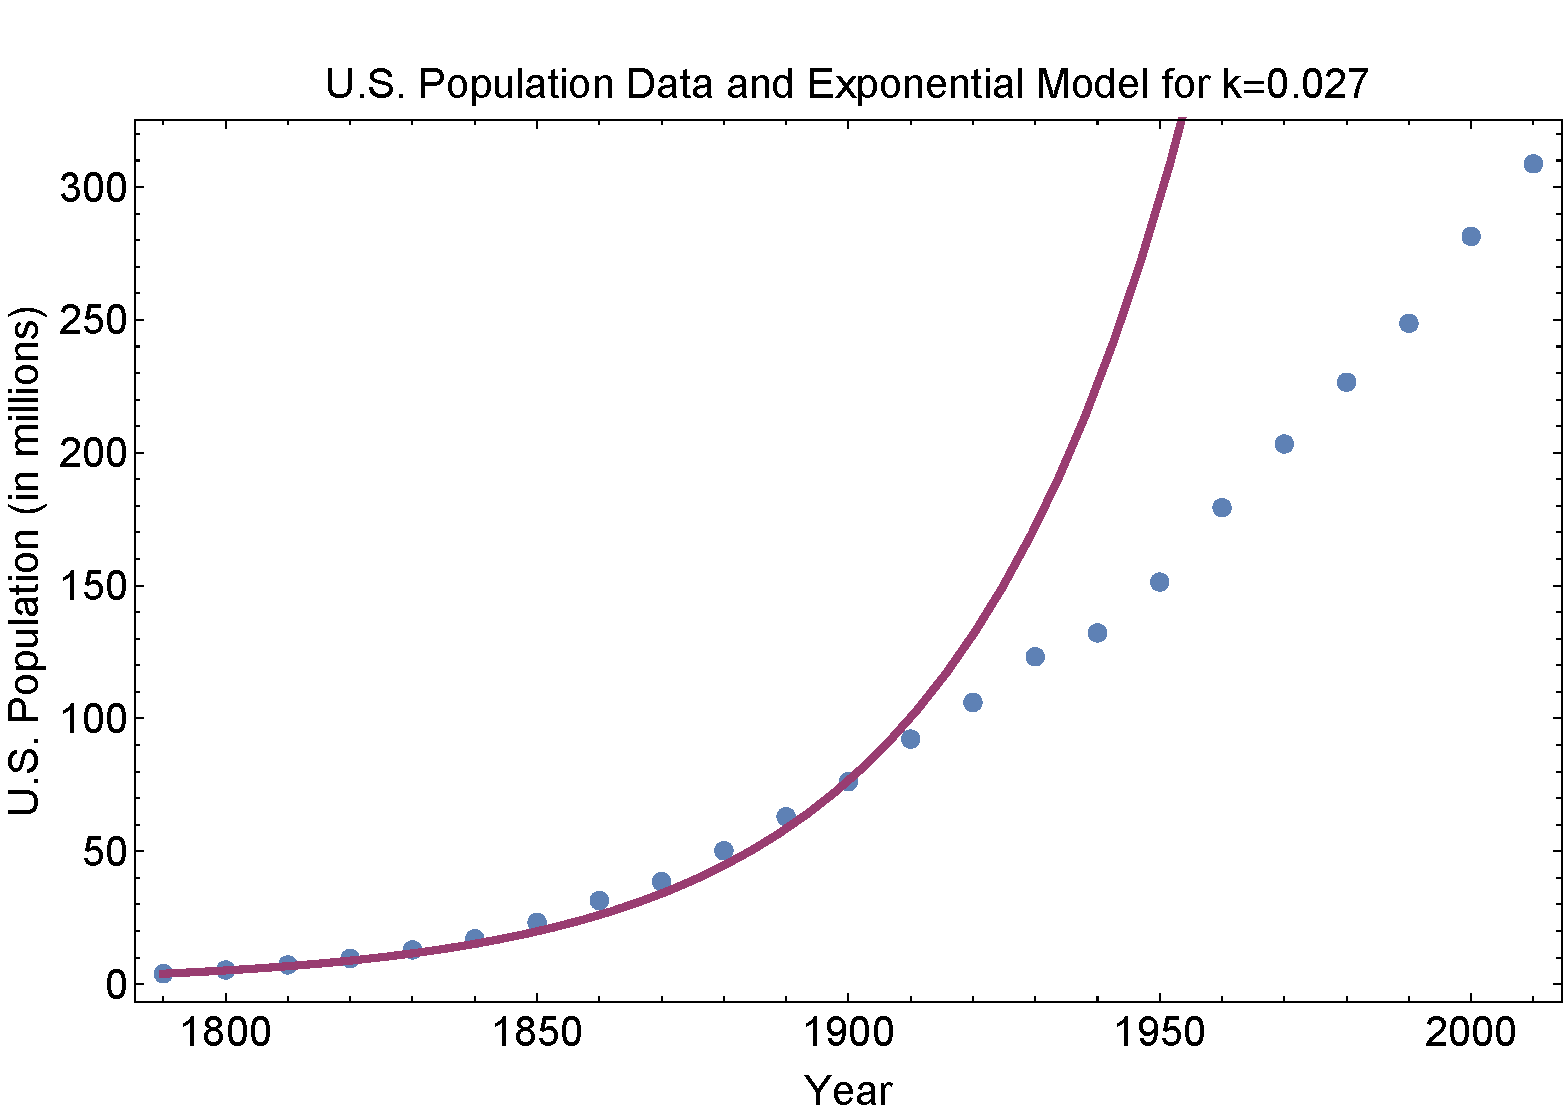
\includegraphics[width=3.2in]{exponentialmodel.pdf}&
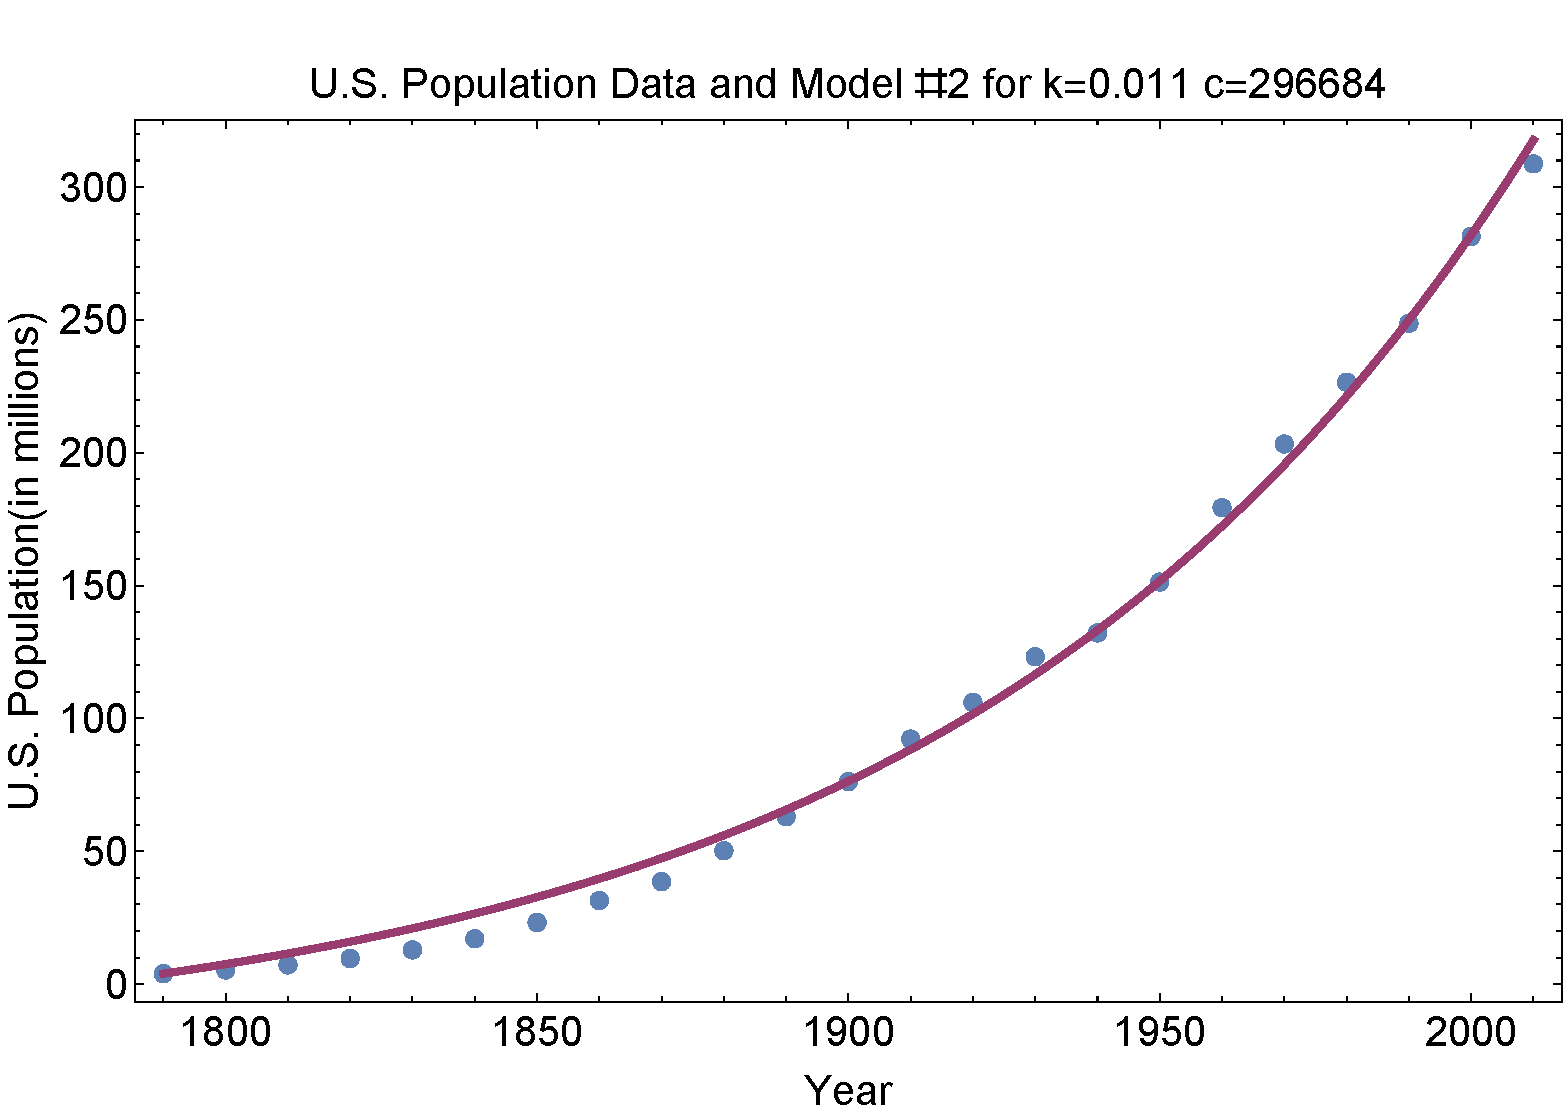
\includegraphics[width=3.2in]{immigrationmodel.pdf}\\
\multicolumn{2}{c}{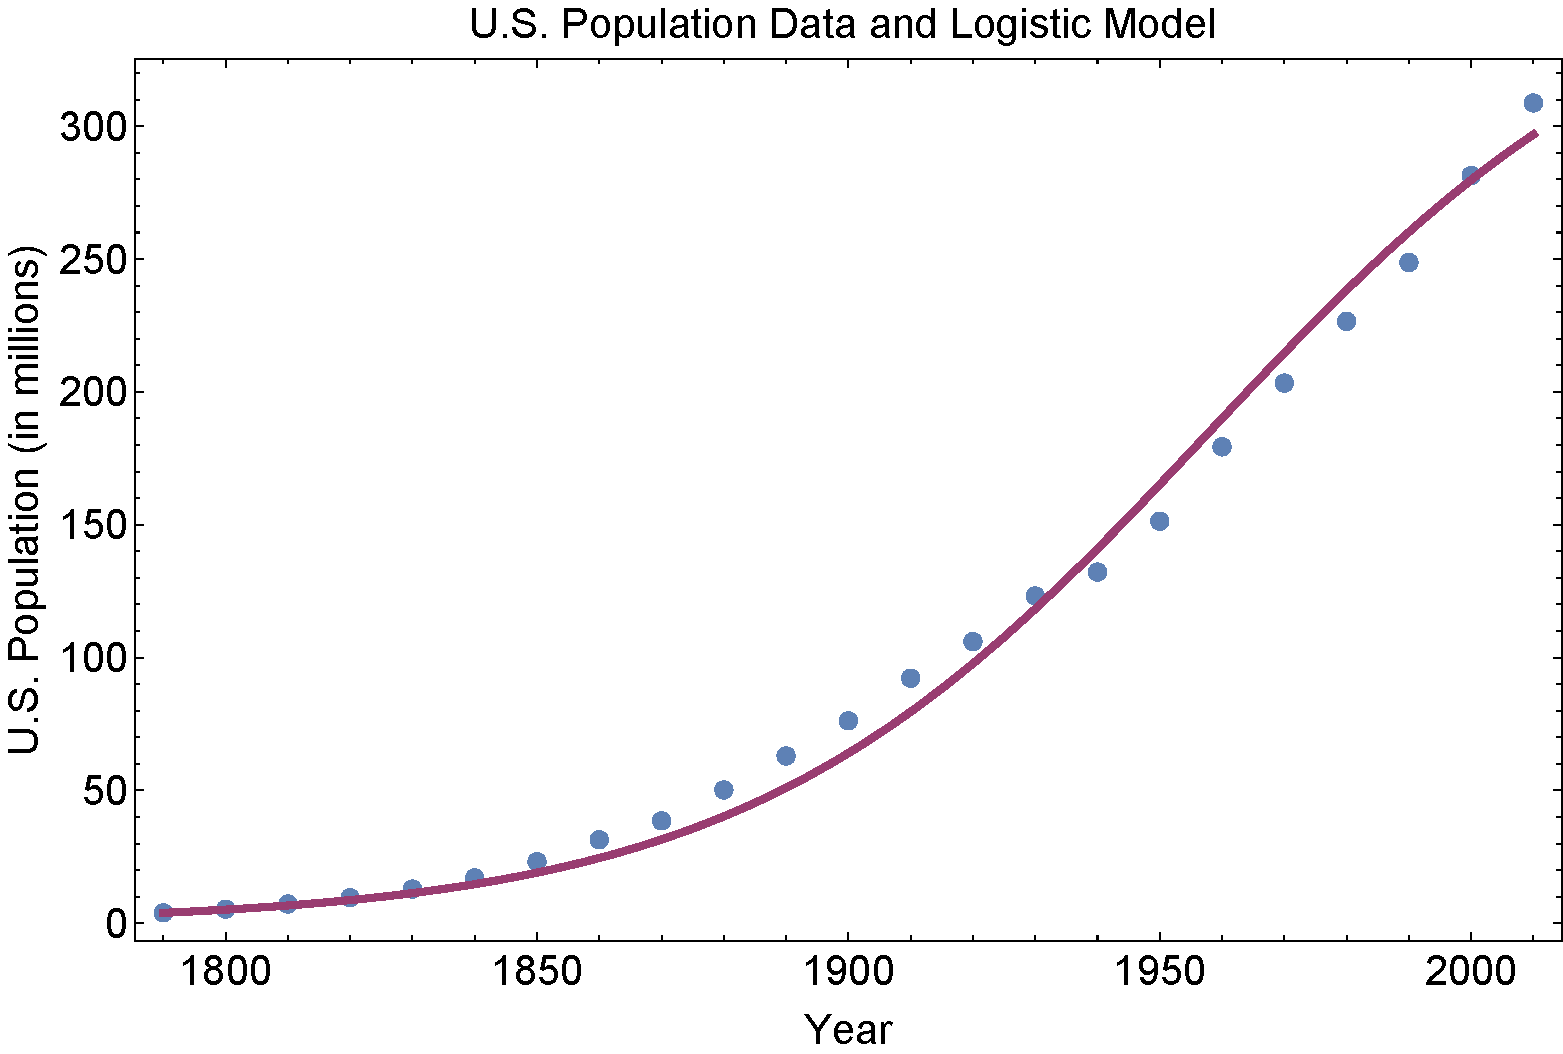
\includegraphics[width=3.2in]{LogisticModel.pdf}}
\end{tabular}
\end{center}
\end{enumerate}
\end{document}  
  
 
